We now present an inclusive study performed at NLO QCD for the EW component, namely the order $\mathcal{O}(\alphas\alpha^6)$.

According to the results shown in Sec.~\ref{subsec:LOinclusive}, the VBS approximation at LO fails in the region $m_{\Pj\Pj} < 200$ GeV, $|\Delta y_{\Pj\Pj}| < 2$.
For the inclusive region (see Eq.~\eqref{eq:inclusive}), this approximation is good up to $\pm10\%$ apart for large di-jet differences and low di-jet invariant mass.
It is therefore interesting to check how good this approximation performs at NLO.
Thus, we impose the same kinematic cuts shown in Sec.~\ref{subsec:inputpar} and apply the VBS cuts of Eq.~\eqref{eq:inclusive}.

We compare three different predictions at NLO QCD: 
the VBS approximation ($|t|^2+|u|^2$) implemented in {\sc Bonsay}, the VBS approximation with the $s$-channel contributions ($|s|^2+|t|^2+|u|^2$) from {\sc VBFNLO}, and the full computation.
The full computation employs full matrix elements meaning that $t/u/s$ interferences, factorisable, and non-factorisable QCD corrections as well as EW corrections to the order $\mathcal{O}(\alphas \alpha^6)$ are included.
% This means that in order to cancel all IR singularities, also EW correction to the $\mathcal{O}(\alphas\alpha^5)$ interference have to be included \cite{Biedermann:2016yds}.
The total cross sections within the above mentioned kinematic cuts are shown in Tab.~\ref{tab:crosssecINCLUSIVE}.

\begin{table}[h!]
\centering
\begin{tabular}{c|c|c}
Prediction & $\sigma_{\textrm{tot}}\,[\textrm{fb}]$ & $\delta [\%]$ \\
\hline
\hline
full &  $1.733\phantom{0} \pm 0.002\phantom{0}$ & - \\
\hline
$|t|^2 + |u|^2$ & $1.6292 \pm 0.0001$  &  $-6$ \\
\hline
$|s|^2 + |t|^2 + |u|^2$ & $1.7780 \pm 0.0001$  & $+2$
\end{tabular}
\caption{
Total cross sections at NLO QCD \emph{i.e.}\ at order $\mathcal{O}(\alphas\alpha^6)$ for the full computation and two approximations.
In addition to the cuts of Sec.~\ref{subsec:inputpar}, the VBS cuts take the values: $m_{\Pj\Pj}>200 \GeV$ and $|\Delta y_{\Pj\Pj}|>2$.}
\label{tab:crosssecINCLUSIVE}
\end{table}

The VBS approximation for NLO QCD predictions (labelled by $|t|^2 + |u|^2$) is lower by about $6\%$ with respect to the full calculation.
The inclusion of $s$-channel diagrams improves the approximate prediction down to a slight excess at the $2\%$-level.

These differences are much more evident in differential distributions.
In Fig.~\ref{fig:mjjdyjj_1d_1}, we show the distributions in the di-jet invariant mass $m_{\Pj\Pj}$ and rapidity separation $|\Delta y_{\Pj\Pj}|$.
For large $m_{\Pj\Pj}$ and large $|\Delta y_{\Pj\Pj}|$, as expected, the VBS approximation is performing well and its $s$-channel extension agree with the full calculation within $10\%$ per cent.
% On the other hand, for low invariant and low rapidity separation the the VBS approximation is failing at a level of at least $30\%$.
% In this very same region, the VBS approximation with $s$-channel is good within $10\%$.
This is in contrast with the region  $200 \GeV < m_{\Pj\Pj} < 500 \GeV$ and $2<|\Delta y_{\Pj\Pj}|<2.5$, the discrepancy between the $|t|^2 + |u|^2$ approximation and the full computation goes up to $30\%$.
The inclusion of $s$-channels cures partly the discrepancy in this region.
Still, for the very low $m_{\Pj\Pj}$ a difference of about $5\%$ remains \MP{To be checked the exact numerical value in data}\GP{Checked in the data}.
This might indicate that interference contributions and/or non-factorisable QCD corrections play a non-negligible role in this phase-space region.

In order to investigate further the jet-pair kinematics, we look at the double-differential distribution in the variables $m_{\Pj\Pj}$ and $\Delta y_{\Pj\Pj}$.
In particular, we compute in each bin the ratio of the approximated cross sections over the full one.
In Fig.~\ref{fig:ratio2d_NLO} we show the ratio $\sigma(|t|^2 + |u|^2)/\sigma(\textrm{full})$ and $\sigma(|s|^2+|t|^2 + |u|^2)/\sigma(\textrm{full})$, in the left and right plot respectively.


\begin{figure*}[hbt]
\centering
{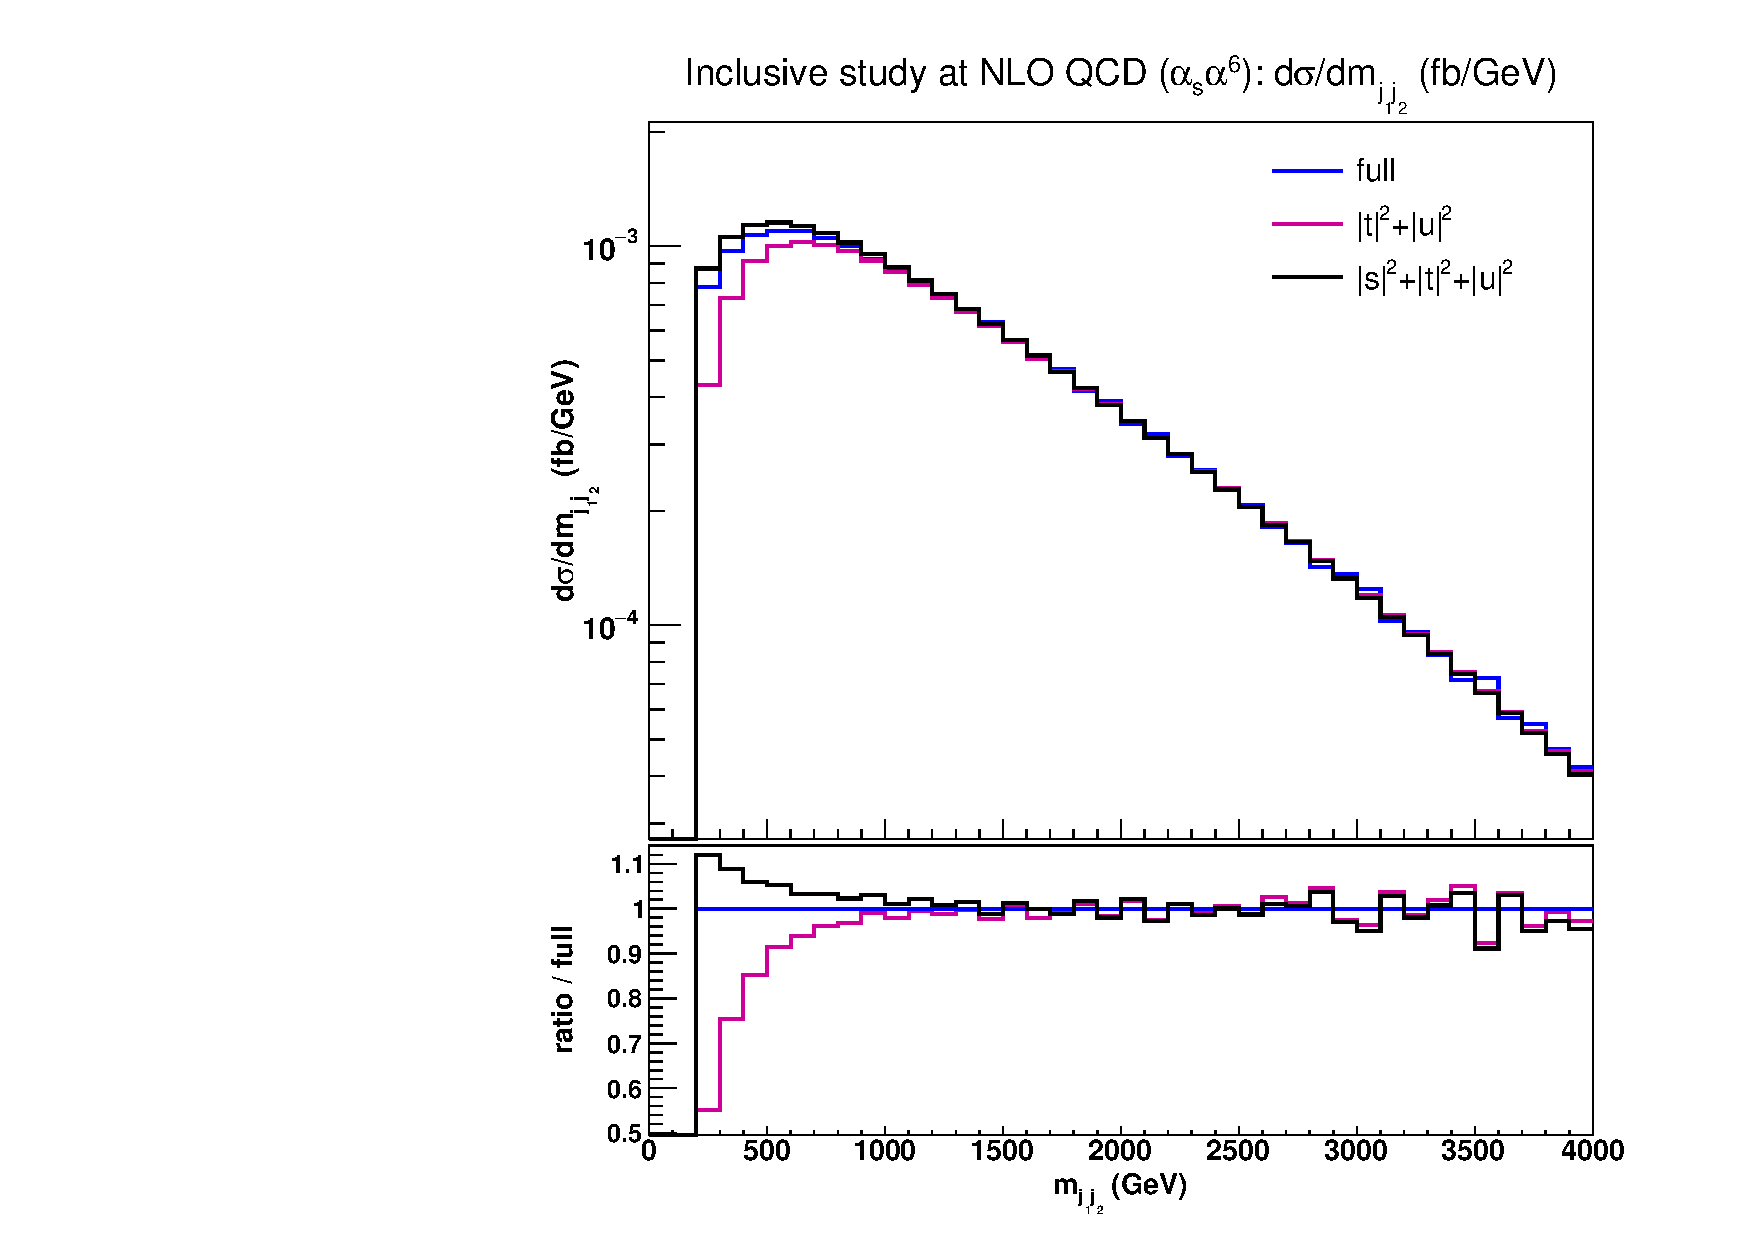
\includegraphics[scale=0.35]{figures/scanfigures/mjj_nlo.pdf}}
{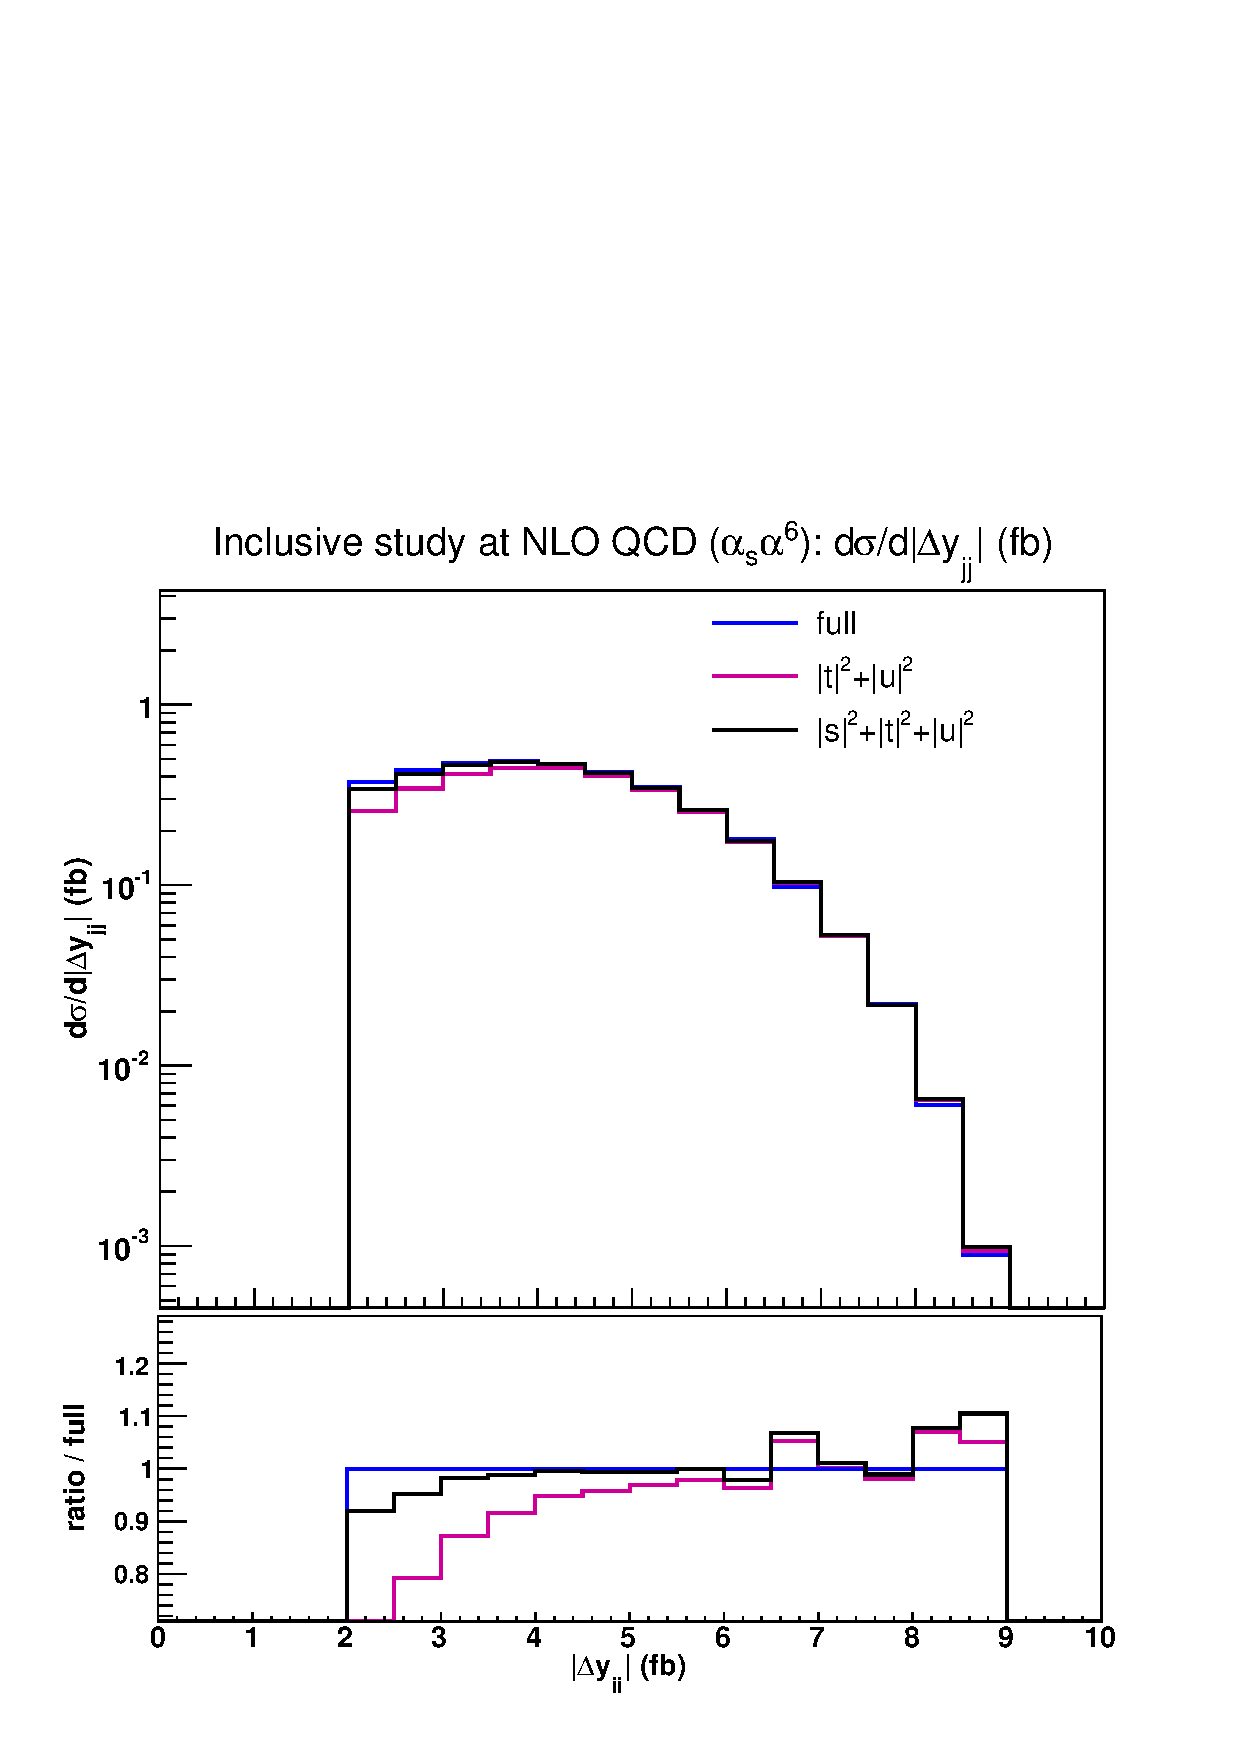
\includegraphics[scale=0.35]{figures/scanfigures/dyjj_nlo.pdf}}
\caption{
Differential distributions in the di-jet invariant mass (left) and the rapidity-separation of the two tagging jets (right) at NLO QCD \emph{i.e.}\ at order $\mathcal{O}(\alphas\alpha^6)$ for the full computation and two approximations.
The upper plots provide the absolute value for each prediction while the lower plots presents all predictions normalised to {\sc MoCaNLO}+{\sc Recola} which is one of the full predictions.
In addition to the cuts of Sec.~\ref{subsec:inputpar}, the VBS cuts take the values: $m_{\Pj\Pj}>200 \GeV$ and $|\Delta y_{\Pj\Pj}|>2$.} 
\label{fig:mjjdyjj_1d_1}
\end{figure*}


\begin{figure*}[hbt]
\centering
{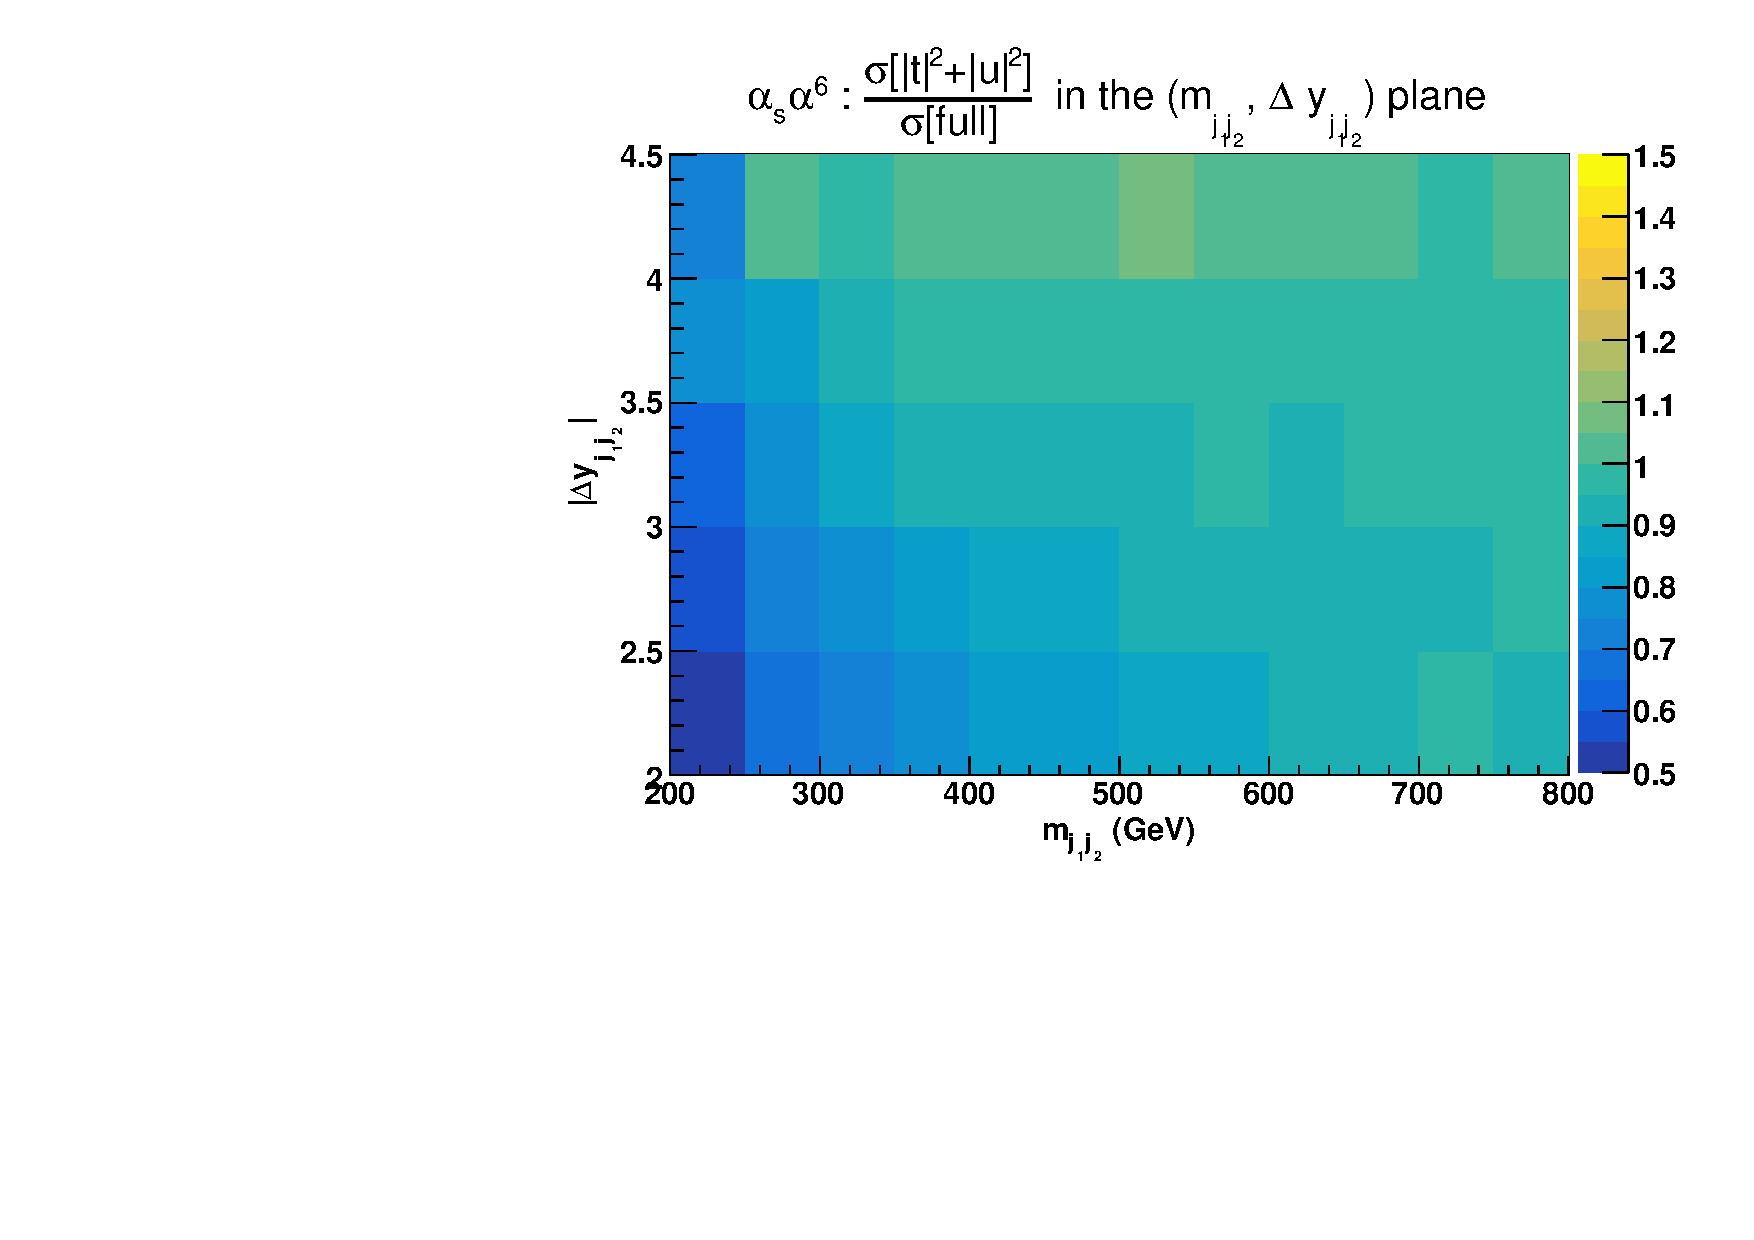
\includegraphics[scale=0.395]{figures/scanfigures/a6as_vbfnloVSrecola_tu.pdf}}
{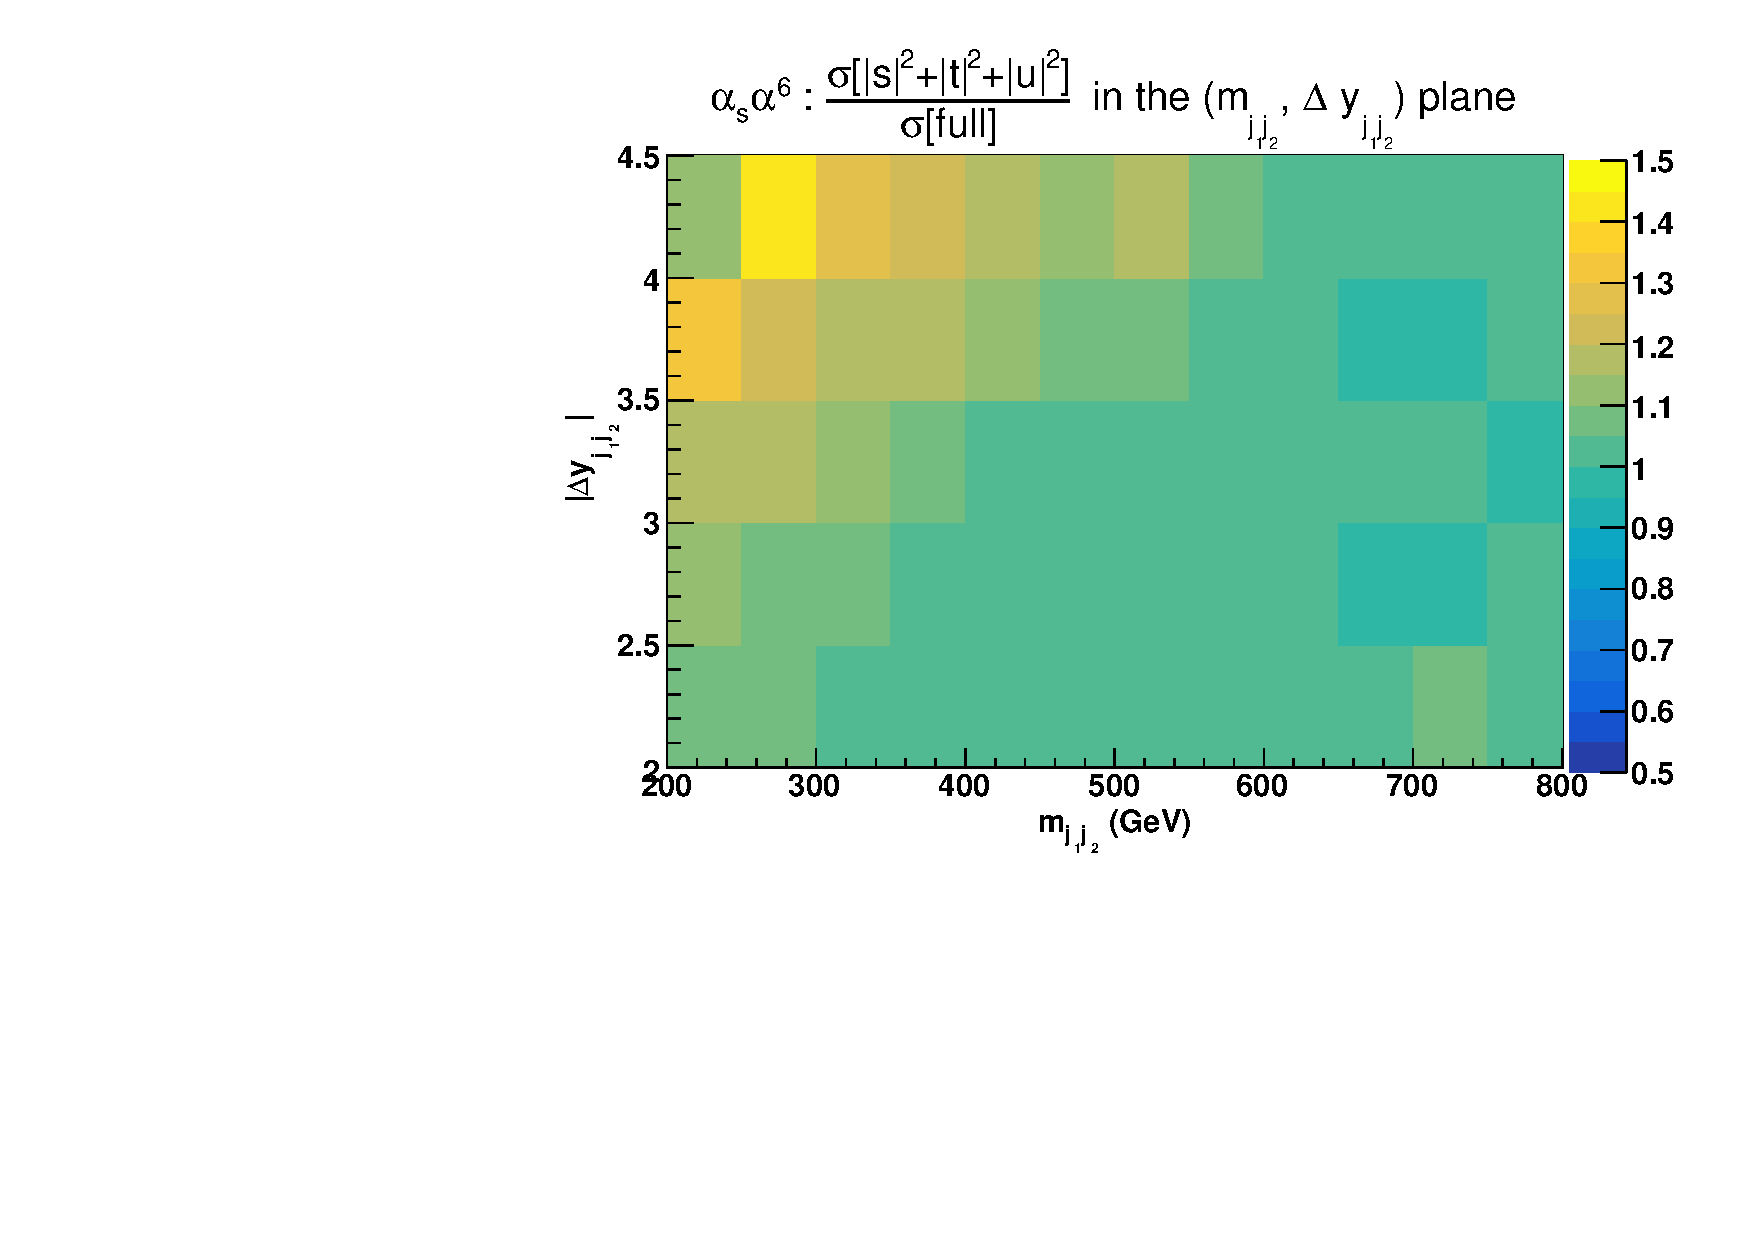
\includegraphics[scale=0.395]{figures/scanfigures/a6as_vbfnloVSrecola_stu.pdf}}
\caption{Ratio of cross sections per bin in the plan $\left(m_{\Pj\Pj}, |\Delta y_{\Pj\Pj}| \right)$ at NLO QCD \emph{i.e.}\ at order $\mathcal{O}(\alphas\alpha^6)$ for the VBS approximation over the full computation.
Ratio of approximated squared amplitudes over the full matrix element.
The approximated squared amplitudes are computed as $|\mathcal{A}|^2 \sim |t|^2 + |u|^2$ (left) and $|\mathcal{A}|^2 \sim |s|^2 + |t|^2 + |u|^2$ (right)
In addition to the cuts of Sec.~\ref{subsec:inputpar}, the VBS cuts take the values: $m_{\Pj\Pj}>200 \GeV$ and $|\Delta y_{\Pj\Pj}|>2$.}
\label{fig:ratio2d_NLO}
\end{figure*}
%
% \begin{figure}[hbt]
% \centering
% {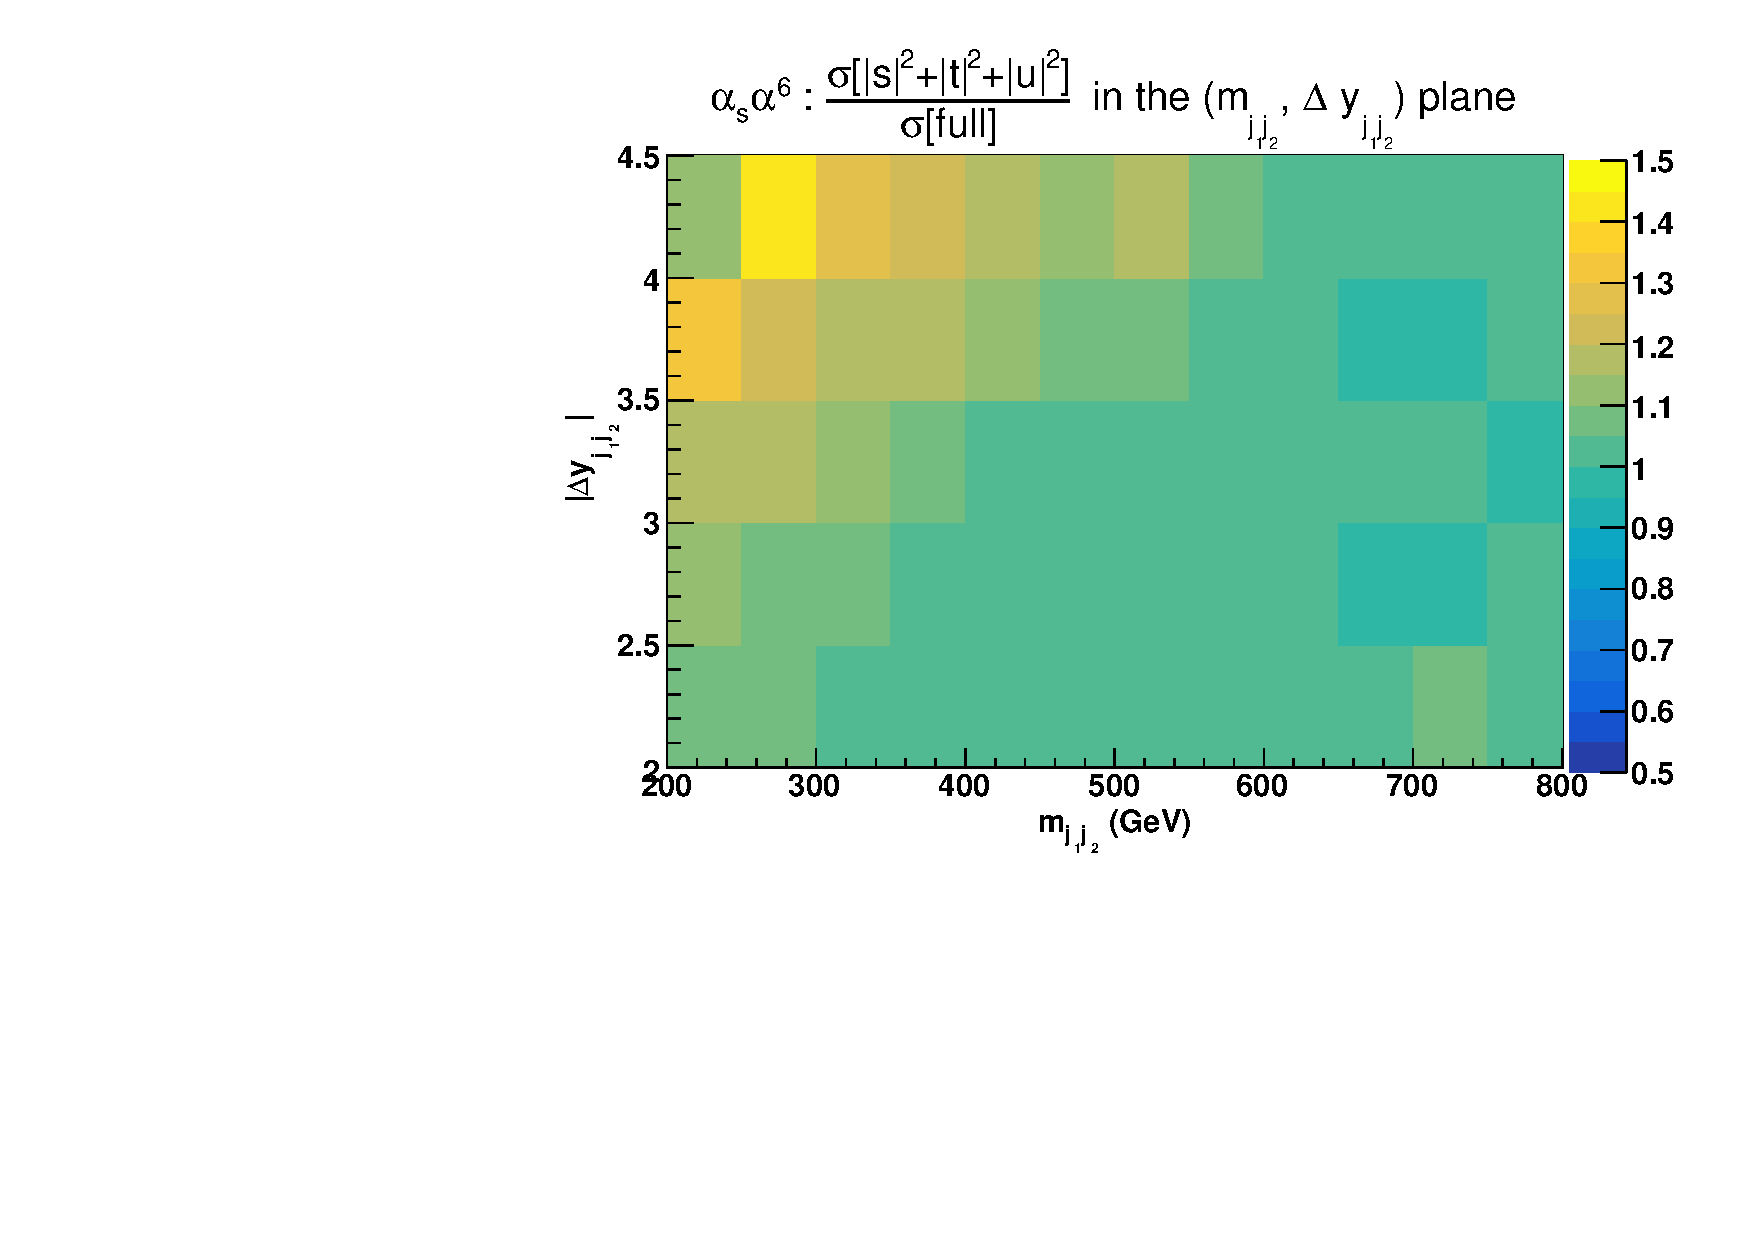
\includegraphics[scale=0.39]{figures/scanfigures/a6as_vbfnloVSrecola_stu.pdf}}
% \caption{Ratio of cross sections (fb) per bin in the plan $\left(m_{\Pj\Pj}, |\Delta y_{\Pj\Pj}| \right)$ at NLO QCD \emph{i.e.}\ at order $\mathcal{O}(\alphas\alpha^6)$ for the VBS approximation with $s$-channel contributions over the full computation.
% In addition to the cuts of Sec.~\ref{subsec:inputpar}, the VBS cuts take the values: $m_{\Pj\Pj}>200 \GeV$ and $|\Delta y_{\Pj\Pj}|>2$.}
% \label{fig:mjjdyjj_2d_NLO}
% \end{figure}

As expected, in the low invariant mass--low rapidity separation region of the jet pair ($200 \GeV < m_{\Pj\Pj} < 500 \GeV$, $2<|\Delta y_{\Pj\Pj}|<2.5$) the VBS approximation fails significantly ($30\%$ discrepancy).
The inclusion of the $s$-channel brings the difference down to $5\%$ \MP{To be checked the exact numerical value in data}\GP{Checked in the data: respectively the two numbers are 29.4\% and 5.4\% in terms of integrated cross-section in this region}.
However, the positive discrepancy shown in the low $m_{\Pj\Pj}$ region (black curve on the upper plots of Fig.~\ref{fig:mjjdyjj_1d_1}) can be traced back to the low $m_{\Pj\Pj}$, large $\Delta y_{\Pj\Pj}$ region of Fig.~\ref{fig:ratio2d_NLO}.
% In this region, the two leading jets have soft transverse momenta, according to the following low-angle approximation
% 
% \begin{equation}
% \begin{split}
% m_{\Pj_i\Pj_j}^2 &= 2\,\ptsub{\Pj_i}\ptsub{\Pj_j}\,(\cosh \Delta y_{\Pj_i\Pj_j} - \cos \Delta\phi_{\Pj_i\Pj_j}) \\
% &\approx 2\,\ptsub{\Pj_i}\ptsub{\Pj_j}\,\cosh \Delta y_{\Pj_i\Pj_j} \,\,.
% \end{split}
% \end{equation}

The same positive discrepancy for the $|s|^2 + |t|^2 + |u|^2$ approximation, can be seen in the low transverse-momentum region of the leading jet in the upper plot of Fig.~\ref{fig:mjjdyjj_1d_2}.
In the large invariant mass--small rapidity separation region of Fig.~\ref{fig:ratio2d_NLO}, discrepancies at the level of $15\%$ are present. This can be traced back to the large $\pt$ and central rapidity region of the leading jets kinematics, shown in Fig.~\ref{fig:mjjdyjj_1d_2}.{\bf GP: should think again about it, in the lights of the new high stat Recola results. The discrepancy is no more negative in the large pt region.}
For such distributions, despite the $s$-channel inclusion, the discrepancy between the approximated and full result is about $5-10\%$.
In the VBS signal-region the VBS approximation shows a good agreement with the full calculation as documented in details below.

\begin{figure*}[hbt]
\centering
{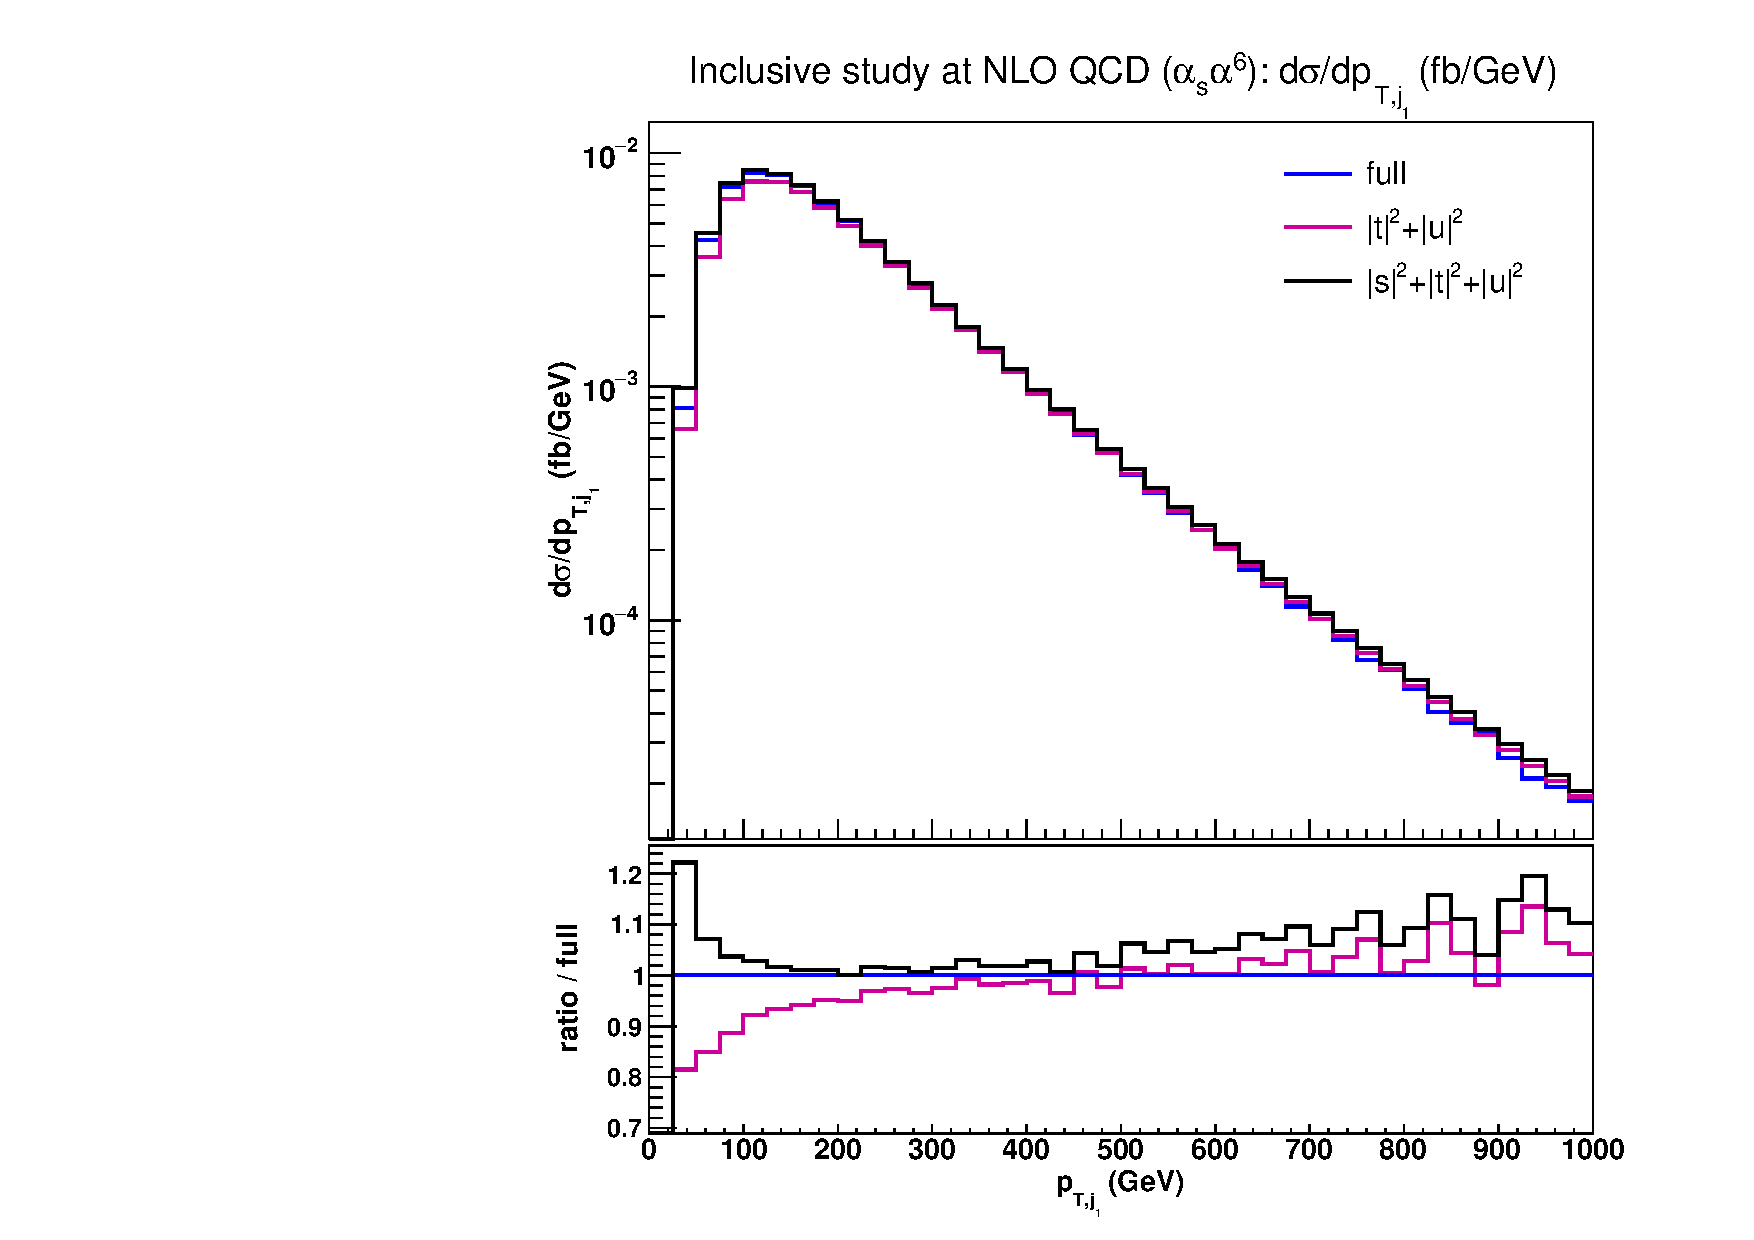
\includegraphics[scale=0.35]{figures/scanfigures/ptj1_nlo.pdf}}
{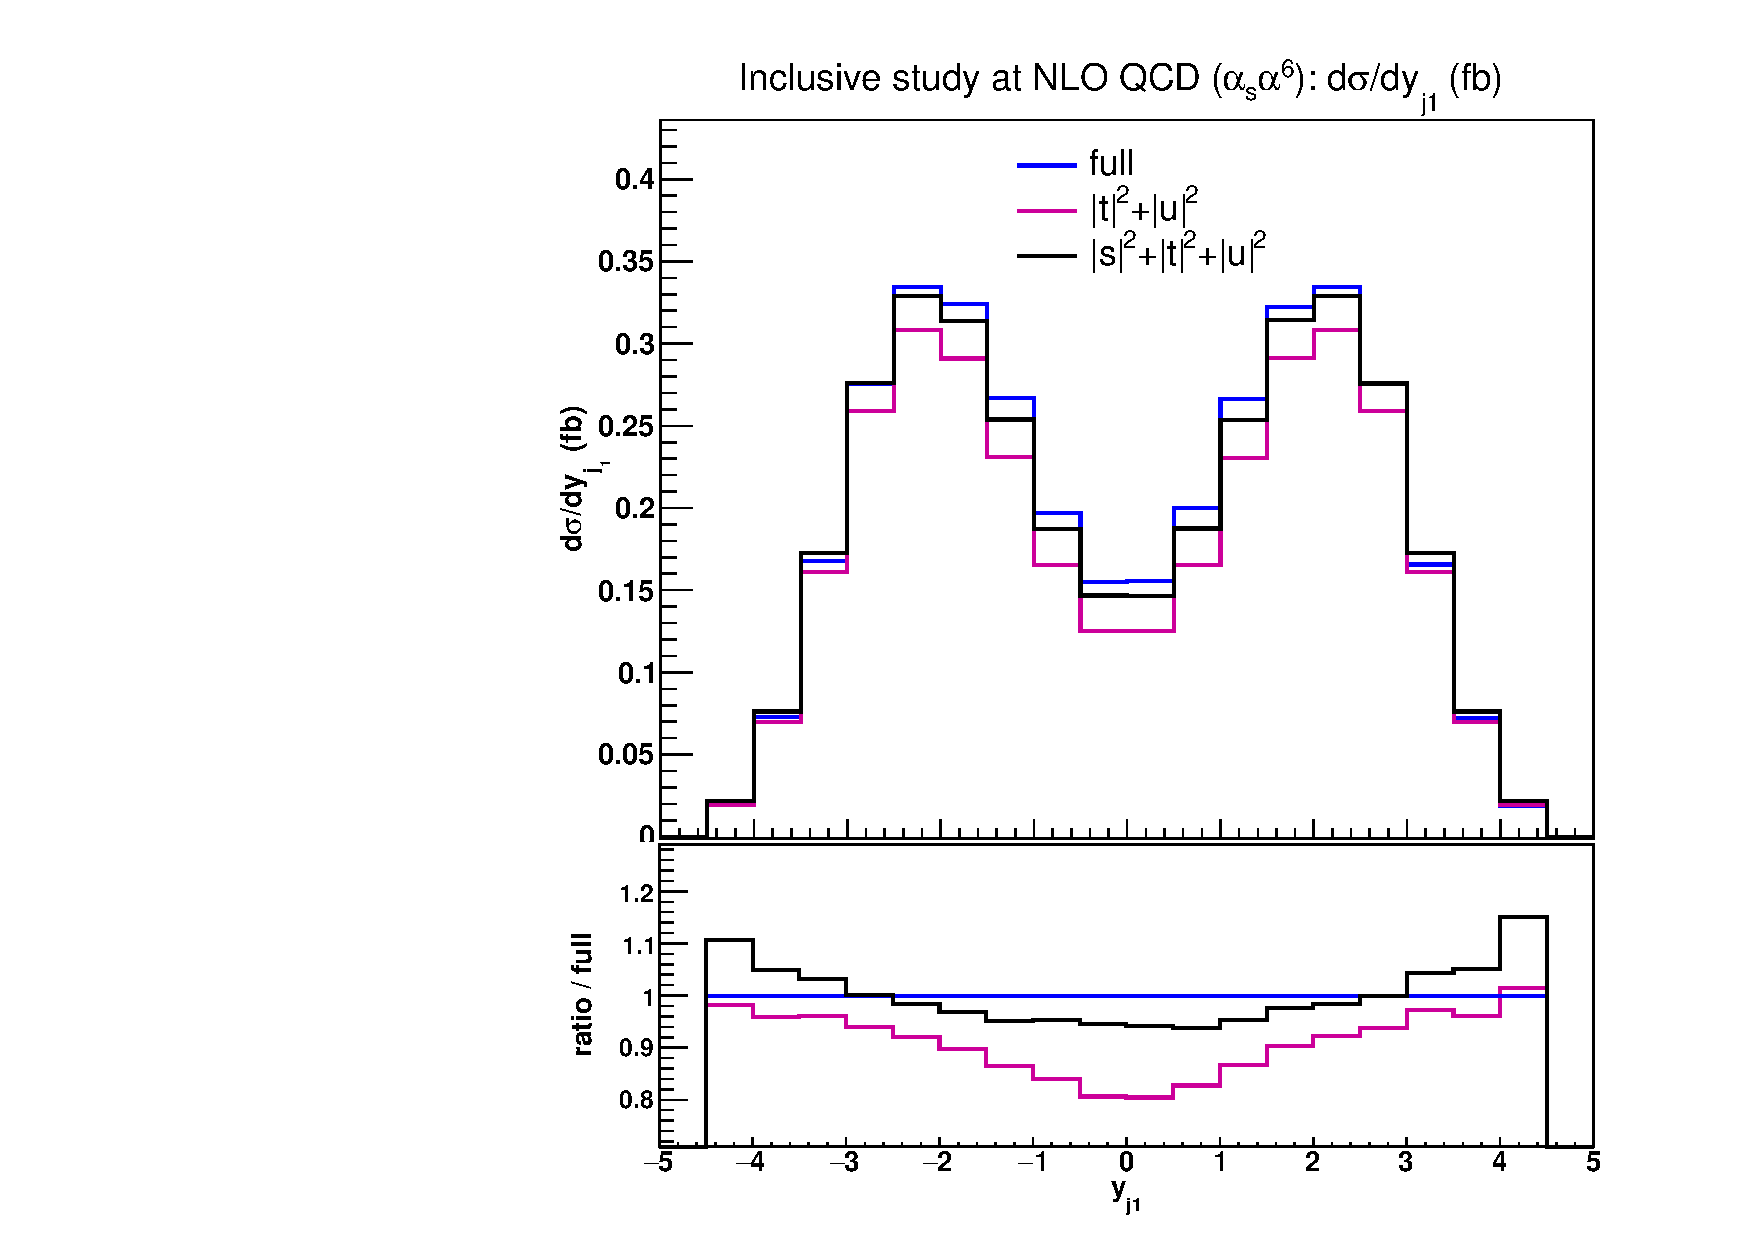
\includegraphics[scale=0.35]{figures/scanfigures/yj1_nlo.pdf}}
\caption{Differential distributions in the transverse momentum (left) and rapidity of the hardest tagging jet (right) at NLO QCD \emph{i.e.}\ at order $\mathcal{O}(\alphas\alpha^6)$ for the full computation and two approximations.
The upper plots provide the absolute value for each prediction while the lower plots presents all predictions normalised to {\sc MoCaNLO}+{\sc Recola} which is one of the full predictions.
In addition to the cuts of Sec.~\ref{subsec:inputpar}, the VBS cuts take the values: $m_{\Pj\Pj}>200 \GeV$ and $|\Delta y_{\Pj\Pj}|>2$.} 
\label{fig:mjjdyjj_1d_2}
\end{figure*}

Concerning leptonic observables, we show in Fig.~\ref{fig:mjjdyjj_1d_3} the distributions of the lepton-lepton invariant mass and of the Zeppenfeld variable of the electron, defined as
%
\begin{equation}
%  z_{\Pe^+} = \frac{y_{\Pe^+}-\frac{y_{\Pj_1}+y_{\Pj2}}2}{|y_{\Pj_1}-y_{\Pj_2}|} \,.
  z_{\Pe^+} = \frac{y_{\Pe^+}-\frac{y_{\Pj_1}+y_{\Pj2}}2}{|\Delta y_{jj}|} \,.
  \label{eq:Zeppenfeld}
\end{equation}
%
Analogous definitions will later also be used for the Zeppenfeld variable of the muon and of the third jet.
%
\begin{figure*}[hbt]
\centering
{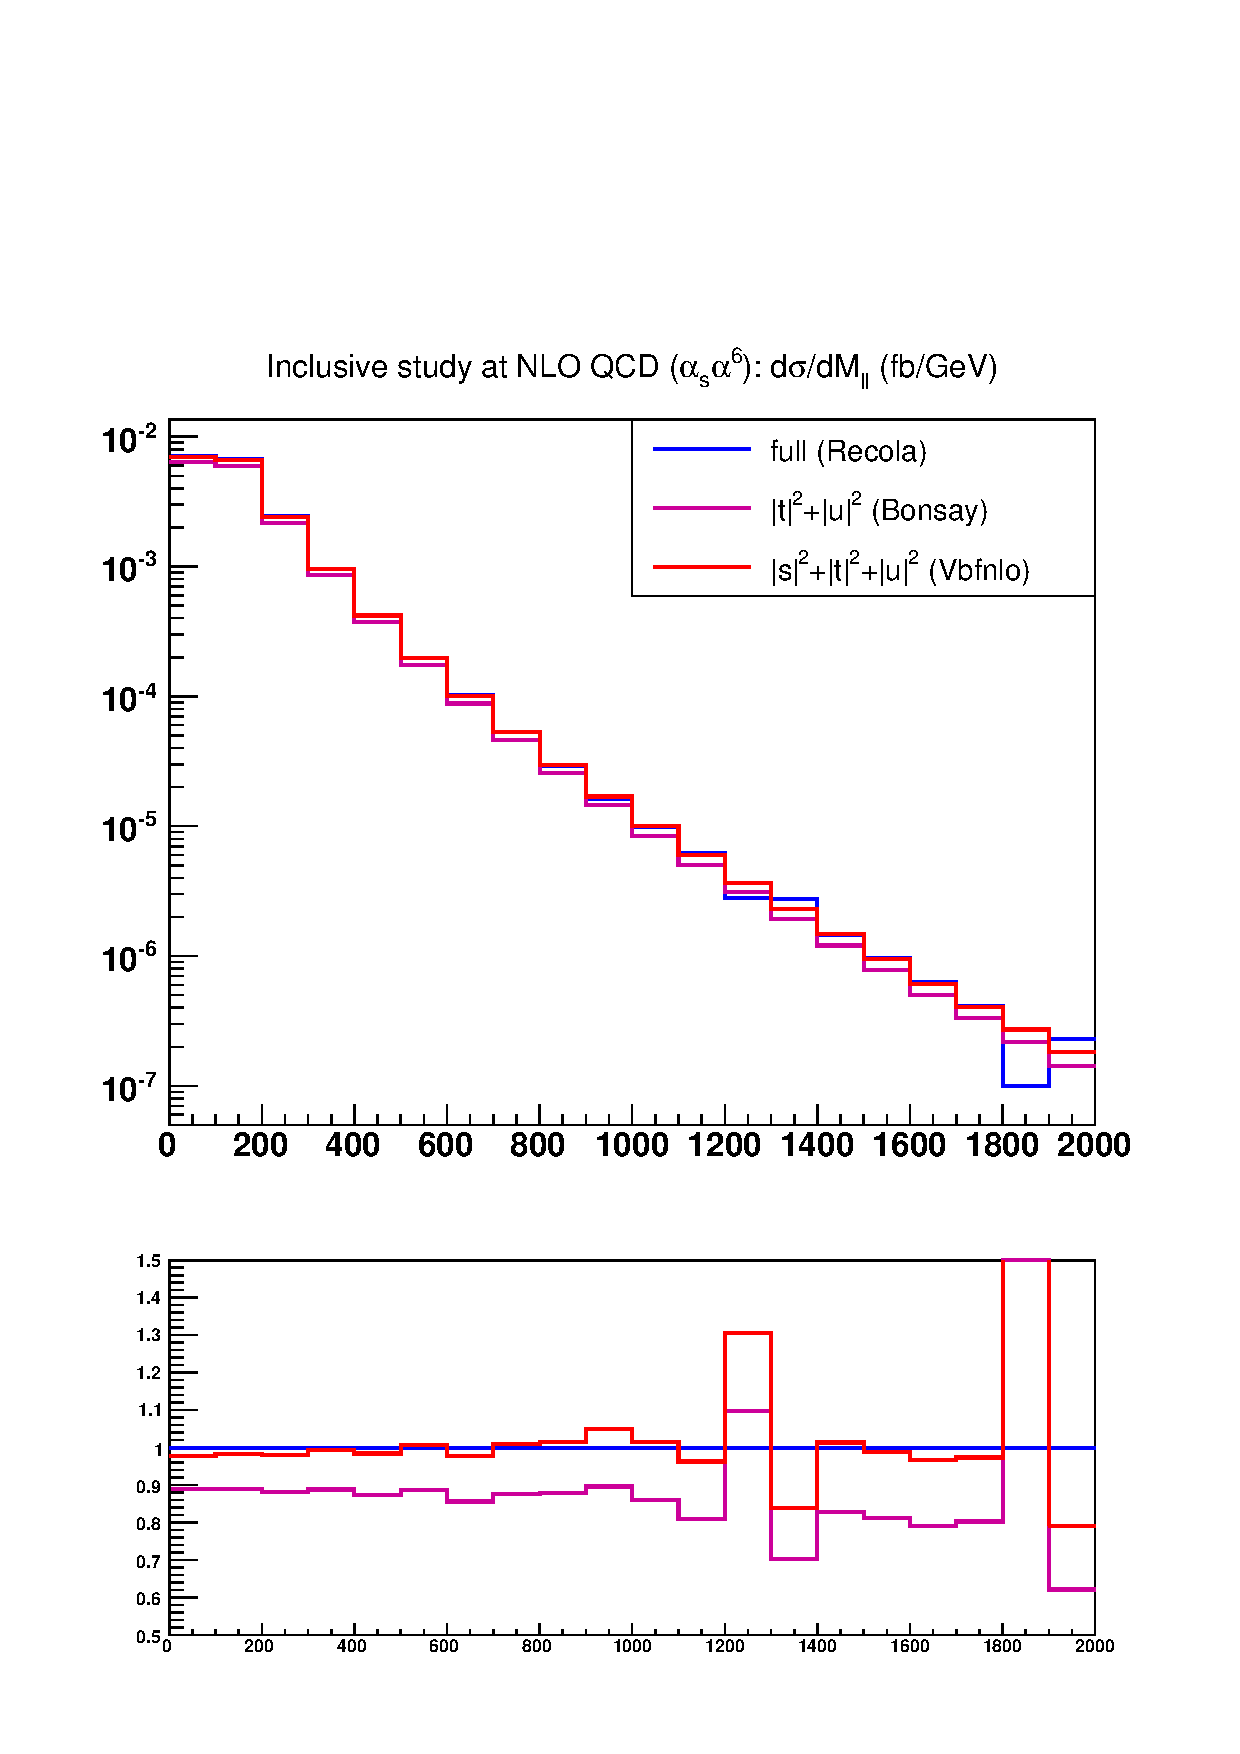
\includegraphics[scale=0.35]{figures/scanfigures/mll_nlo.pdf}}
{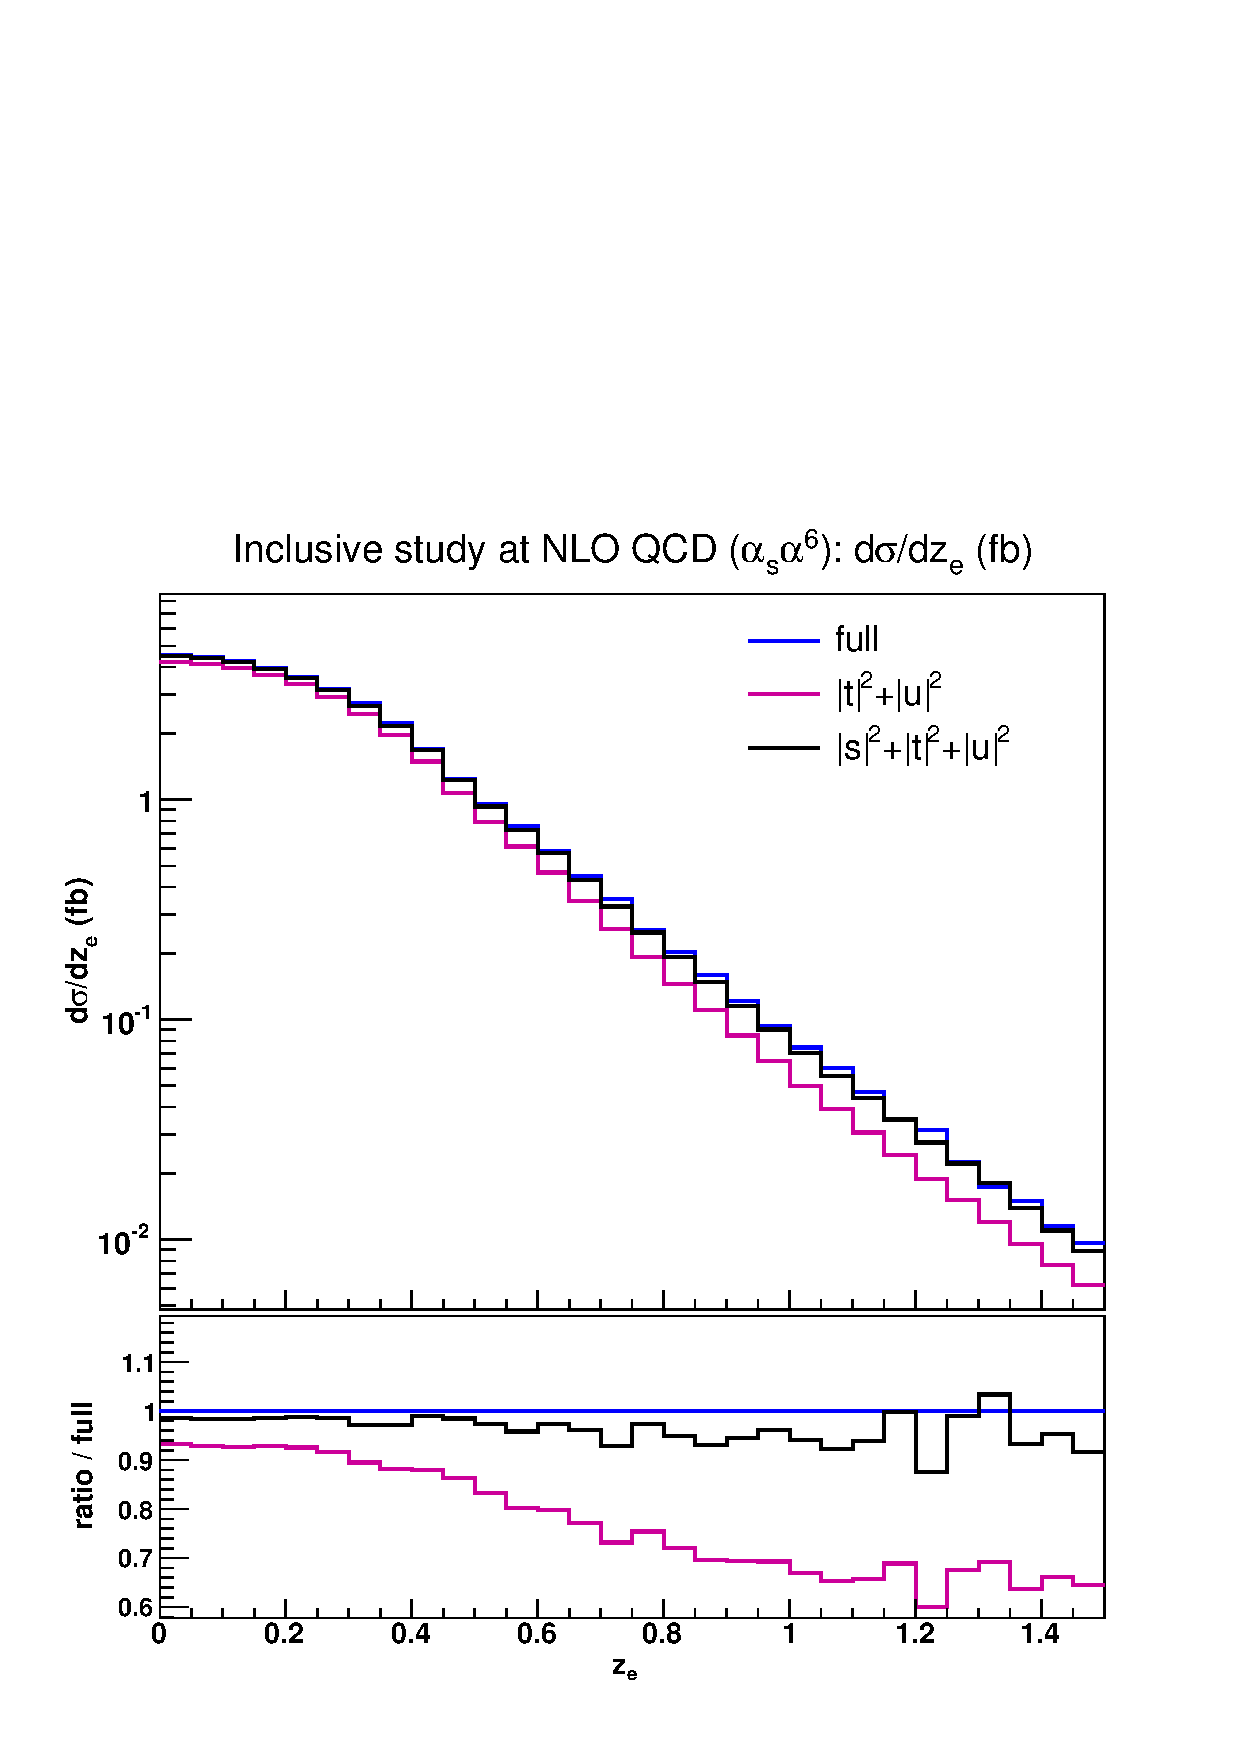
\includegraphics[scale=0.35]{figures/scanfigures/zel_nlo.pdf}}
\caption{Differential distributions in the lepton-lepton invariant mass (left) and the electron Zeppenfeld variable (right) at NLO QCD \emph{i.e.}\ at order $\mathcal{O}(\alphas\alpha^6)$ for the full computation and two approximations.
The upper plots provide the absolute value for each prediction while the lower plots presents all predictions normalised to {\sc MoCaNLO}+{\sc Recola} which is one of the full predictions.
In addition to the cuts of Sec.~\ref{subsec:inputpar}, the VBS cuts take the values: $m_{\Pj\Pj}>200 \GeV$ and $|\Delta y_{\Pj\Pj}|>2$.} 
\label{fig:mjjdyjj_1d_3}
\end{figure*}
%
The {\sc VBFNLO} result for the $e^+\mu^+$ invariant mass agrees rather well with the full curve, obtained from {\sc MoCa\-NLO+Recola}.
The prediction from {\sc Bonsay} is about $10\%$ lower for $m_{e^+\mu^+}<1200 \GeV$; this discrepancy reaches about $20\%$ in the very high mass region. 
%The discrepancies are roughly constant over the whole spectrum.
Instead, the right panel of Fig.~\ref{fig:mjjdyjj_1d_3} clearly shows that the Zeppenfeld variable of the positron $z_e$ is strongly affected by the exclusion of $s$-channels, with increasing negative discrepancy with respect to the full result at large values (up to $30\%$ for $z_{e^+}>1.2$). Including $s$-channels makes this discrepancy become positive, but smaller than $10\%$ over the whole spectrum.
The muon observable $z_{\mu}$ behaves identically to the electron one, $z_e$.

In conclusion, both the loose minimum di-jet invariant mass cut and the inclusion of QCD radiative correction make the $s$-channel contributions less suppressed than at LO, making their inclusion mandatory, in order to provide trustworthy predictions at NLO accuracy.
Nevertheless, interferences and non-factorizable QCD corrections should be included to reduce the discrepancies down to about $1\%$, mainly in inclusive analyses.
Instead, the VBS approximation at NLO provides a good approximation of full calculations in the kinematic region where VBS contributions are dominant ($M_{\Pj\Pj} \gtrsim 600 \GeV$, $|\Delta y_{\Pj\Pj}| \gtrsim 3$), for both total cross section and differential distributions.
